\documentclass[conference,a4paper]{IEEEtran}

\usepackage[T1]{fontenc}
\usepackage[utf8]{inputenc}
\usepackage[spanish,es-tabla,es-nodecimaldot,es-noshorthands]{babel}
\usepackage{graphicx}
\usepackage{booktabs}
\usepackage{array}
\usepackage{amsmath}
\usepackage{amssymb}
\usepackage{cite}
\usepackage{xurl}
\usepackage[table]{xcolor}
\usepackage{tikz}
\usepackage[hidelinks]{hyperref}

\graphicspath{{img/}}

\definecolor{deepnavy}{HTML}{042347}
\definecolor{modernteal}{HTML}{168B8D}
\definecolor{plgray}{HTML}{F5F5F5}
\definecolor{midgray}{HTML}{CCCCCC}

\renewcommand{\IEEEkeywordsname}{Palabras clave}

% Celdas de la tabla comparativa
\newcommand{\si}{\checkmark}
\newcommand{\pa}{$\sim$}
\newcommand{\no}{--}

\begin{document}

\title{ParkLink: Plataforma de microservicios para la reserva anticipada de estacionamiento urbano y el uso colaborativo de cocheras}

\author{\IEEEauthorblockN{Thiago Fernando Baez, Santiago Domínguez, Facundo Luzzi, Santiago Jorge Varga}
\IEEEauthorblockA{\textit{Facultad de Ingeniería}\\
\textit{Universidad de Buenos Aires (FIUBA)}\\
Buenos Aires, Argentina\\
\{tbaez, sadominguez, fluzzi, svarga\}@fi.uba.ar}}

\maketitle

%================================================================
\begin{abstract}
El siguiente trabajo presenta ParkLink, un mercado digital de dos lados que conecta a conductores que necesitan estacionar en la Ciudad Autónoma de Buenos Aires con propietarios de cocheras particulares y playas comerciales. La plataforma reformula la búsqueda de estacionamiento, un problema de parada óptima con información incompleta, como una elección simultánea entre opciones visibles, comparables y reservables antes de salir. Se describen la arquitectura de microservicios políglota que la sostiene, las decisiones de diseño que garantizan la consistencia de las reservas ante solicitudes concurrentes, el procesamiento idempotente de pagos y eventos, y la metodología ágil híbrida con la que un equipo de cuatro integrantes la construyó en trece \textit{sprints}. Se reportan los resultados de su validación técnica, con 128 archivos de pruebas automatizadas, y de su validación de producto, mediante una encuesta a 180 potenciales usuarios que arrojó un 70\% de intención de uso regular, un encuentro con un operador comercial del sector y la adecuación a la normativa argentina de defensa del consumidor y protección de datos.
\end{abstract}

\begin{IEEEkeywords}
Estacionamiento urbano, microservicios, mercado de dos lados, parada óptima, búsqueda geoespacial, economía colaborativa.
\end{IEEEkeywords}

%================================================================
\section{Introducción}\label{sec:intro}
%================================================================

\subsection{Contexto y motivación}

La movilidad urbana es uno de los desafíos centrales de las grandes ciudades, y el estacionamiento ocupa en ella un lugar particular: Es el último tramo de casi cualquier viaje en automóvil y, al mismo tiempo, el que menos herramientas tecnológicas ha recibido. Mientras que el transporte de pasajeros o el alojamiento temporario se resolvieron con plataformas que conectan a quien ofrece un recurso con quien lo necesita, en la Ciudad Autónoma de Buenos Aires (CABA), donde circulan a diario alrededor de 1,8~millones de vehículos~\cite{superauto2024,aboy2025movilidad}, el estacionamiento sigue repartido entre canales que no dialogan entre sí: El estacionamiento medido en la vía pública, las playas comerciales a las que se accede sin reserva y los avisos clasificados de cocheras orientados casi exclusivamente al alquiler mensual.

En esa brecha conviven dos ineficiencias. Del lado de la demanda, el conductor no puede saber antes de salir si va a tener dónde estacionar ni cuánto le va a costar. Del lado de la oferta, muchas cocheras residenciales y playas comerciales permanecen ociosas durante buena parte del día porque sus propietarios no disponen de un medio seguro y simple para ofrecerlas por períodos cortos. El problema, por lo tanto, no es la falta de lugares, sino la falta de información y de un canal transaccional confiable que conecte ambos lados.

\subsection{La búsqueda de estacionamiento como problema de parada óptima}

La dificultad que enfrenta el conductor tiene una formulación precisa: Es un problema de parada óptima (\textit{optimal stopping}). En esta familia de problemas, una persona evalúa opciones de a una, en un orden que no controla, y debe decidir en cada momento si acepta la que tiene delante o la descarta, sin posibilidad de recuperarla. En el caso más conocido, el problema de la secretaria, la estrategia óptima elige la mejor opción con una probabilidad de apenas el 37\%~\cite{ferguson1989,christian2016}.

El estacionamiento tiene su propia versión, formulada por MacQueen y Miller~\cite{macqueen1960}: Un conductor avanza hacia su destino, solo ve el lugar que tiene enfrente y no puede volver a uno que dejó pasar. La estrategia óptima es de umbral, es decir, ignorar los lugares libres hasta cierta distancia del destino y tomar el primero disponible a partir de allí; si nueve de cada diez lugares están ocupados, conviene empezar a buscar seis lugares antes~\cite{fergusonstopping}. Las variantes que permiten regresar a un lugar ya visto a cambio de un costo~\cite{tamaki1988} confirman que es la falta de información sobre lo que hay más adelante la que obliga a decidir sin certezas. Lo mismo ocurre con las cocheras y las playas: El conductor las descubre de a una, sin conocer su precio ni su disponibilidad hasta llegar, y ante el apuro termina aceptando la primera opción aceptable.

\subsection{Costo de la búsqueda}

La búsqueda tiene además un costo económico concreto. Con datos de CABA de 2026, se estimó el costo de cada salida sin un lugar asegurado en cuatro componentes (Tabla~\ref{tab:costo}): El tiempo perdido, tomando unos 15~minutos de búsqueda valorizados al salario promedio de la Ciudad~\cite{infobae_salarios_2026}; el combustible consumido en 2 a 3~km de marcha lenta~\cite{economista_nafta_2026}; el valor esperado de una multa por estacionamiento indebido, de \$94.999~ARS, asumiendo una infracción cada 120 salidas~\cite{infobae_multas_2026}; y el sobrecosto de aceptar una cochera sin comparar, dado que la hora varía entre \$6.000 y \$10.000~ARS según la zona y llega a \$20.000~ARS en las de mayor demanda~\cite{iprofesional2026cocheras}.

\begin{table}[!t]
\centering
\caption{Costo estimado por búsqueda de estacionamiento en CABA (2026)}
\label{tab:costo}
\renewcommand{\arraystretch}{1.2}
\begin{tabular}{l r}
\toprule
\textbf{Concepto} & \textbf{Costo (ARS)} \\
\midrule
Tiempo perdido (${\sim}$15 min) & \$3.464 \\
Combustible (${\sim}$0,25 L) & \$556 \\
Riesgo de multa (1 cada 120 salidas) & \$792 \\
Sobrecosto por no comparar (1 cada 10 salidas) & \$800 \\
\midrule
\textbf{Total por búsqueda} & \textbf{\$5.612} \\
\bottomrule
\end{tabular}
\end{table}

\subsection{Objetivos y contribuciones}

El objetivo del trabajo fue diseñar, desarrollar y validar una plataforma que permita a los conductores de CABA buscar, reservar y pagar un lugar con disponibilidad confirmada antes de llegar a destino, y a los propietarios publicar y administrar sus espacios con la confianza de un cobro y una identidad verificados. Las contribuciones de este artículo son las siguientes:

\begin{itemize}
    \item La reformulación de la búsqueda de estacionamiento, de una búsqueda secuencial con información incompleta a una elección simultánea entre opciones visibles y reservables, materializada en un producto funcional.
    \item El diseño de una arquitectura de microservicios políglota con un motor de reservas que admite cocheras de capacidad múltiple sin sobre-reserva ante solicitudes concurrentes, y con procesamiento idempotente de pagos y eventos.
    \item La descripción de una metodología ágil híbrida adaptada a cada fase del proyecto, que permitió el desarrollo en paralelo de ocho componentes a partir de contratos acordados de antemano.
    \item Una validación en tres planos (técnico, de mercado y legal), cuyas fricciones detectadas se tradujeron en decisiones de producto implementadas.
\end{itemize}

El resto del artículo se organiza de la siguiente manera. La Sección~\ref{sec:estado} revisa la literatura y las soluciones existentes. La Sección~\ref{sec:propuesta} presenta la propuesta: El producto, su arquitectura, las decisiones de diseño, la metodología de desarrollo y la estrategia de validación. La Sección~\ref{sec:resultados} informa los resultados obtenidos, y la Sección~\ref{sec:conclusiones} expone las conclusiones y las líneas de trabajo futuro.

%================================================================
\section{Estado del Arte}\label{sec:estado}
%================================================================

\subsection{El costo de la circulación en busca de estacionamiento}

La circulación en busca de estacionamiento (\textit{cruising for parking}) fue estudiada como un fenómeno con efectos agregados sobre el tránsito. Shoup~\cite{shoup2005,shoup2006} relevó estudios realizados en distintas ciudades y estimó que, en las zonas céntricas, en promedio cerca del 30\% del tránsito corresponde a vehículos que buscan dónde estacionar, con el consiguiente aumento de la congestión, el consumo de combustible y las emisiones. Su análisis atribuye el fenómeno a la diferencia de precio entre el estacionamiento en la calle y el de las playas, y propone corregirla mediante la tarificación del espacio público. La perspectiva de la parada óptima~\cite{macqueen1960,tamaki1988}, presentada en la Sección~\ref{sec:intro}, complementa esa explicación desde el lado de la información: Aun con precios correctos, un conductor que solo ve las opciones de a una decide mal. ParkLink actúa sobre esa segunda causa, haciendo visible y reservable la oferta privada que hoy permanece oculta.

\subsection{Soluciones existentes}

\textit{Estacionamiento medido.} Blinkay~\cite{blinkay} es la plataforma de estacionamiento medido más difundida en Argentina y el competidor local más relevante. Permite pagar desde el teléfono el estacionamiento en las zonas reguladas de CABA y de otras ciudades, con una marca consolidada y un flujo de pago validado en el mercado. Sin embargo, opera exclusivamente sobre la vía pública, no ofrece reservas anticipadas y su modelo está atado a contratos municipales, por lo que no contempla cocheras privadas ni playas comerciales.

\textit{Aplicaciones de navegación.} Waze~\cite{waze} y Google Maps~\cite{googlemaps} tienen una penetración altísima e incorporan, en algunos mercados, información aproximada sobre el estacionamiento en determinadas zonas a partir de proveedores externos o de patrones históricos. Esa información es estimativa: No permite reservar, no confirma la disponibilidad real antes de llegar ni integra el pago o la relación con quien ofrece el espacio.

\textit{Clasificados digitales.} Portales como Mercado Libre~\cite{mercadolibre} son el canal más usado por los propietarios particulares para ofrecer cocheras en Argentina. Ofrecen alta visibilidad y bajo costo de publicación, pero están orientados al alquiler mensual, carecen de disponibilidad por horas y de pago dentro de la operación, y dejan la coordinación entre las partes completamente en manos de ellas, con la consiguiente falta de confianza.

\textit{Plataformas internacionales de reserva.} SpotHero y ParkWhiz~\cite{spothero} en Estados Unidos, y EasyPark~\cite{easypark} en más de 20 países europeos, representan el estado del arte de la reserva anticipada: Inventario actualizado, comparación de precios, pago integrado y reseñas. Validan el modelo técnico y comercial a gran escala, pero no operan en Argentina ni en América Latina, se orientan casi exclusivamente a garajes comerciales o a acuerdos con municipios, y no contemplan a los propietarios particulares que quieren aprovechar un espacio ocioso.

\subsection{Síntesis y faltante}

A partir de este relevamiento se definieron cinco criterios de comparación: Presencia en el mercado local, reserva anticipada, disponibilidad real, pago integrado y acceso a la oferta de propietarios particulares. La Tabla~\ref{tab:comparativa} resume cómo los cubre cada actor. Ninguno de los existentes en el mercado argentino los reúne: Blinkay cubre el segmento público regulado sin reservas, los clasificados cubren el alquiler permanente sin transaccionalidad y las referencias internacionales validan el modelo sin operar localmente. ParkLink se construyó para ocupar precisamente ese espacio: Una plataforma transaccional y colaborativa, orientada al estacionamiento de corta y mediana duración en el mercado local.

\begin{table}[!t]
\centering
\caption{Cobertura de los criterios de comparación por actor}
\label{tab:comparativa}
\renewcommand{\arraystretch}{1.2}
\setlength{\tabcolsep}{4pt}
\begin{tabular}{l c c c c c}
\toprule
\textbf{Actor} & \textbf{Local} & \textbf{Reserva} & \textbf{Disp. real} & \textbf{Pago} & \textbf{Particulares} \\
\midrule
Blinkay & \si & \no & \pa & \si & \no \\
Waze / Google Maps & \si & \no & \pa & \no & \no \\
Clasificados & \si & \no & \no & \no & \si \\
SpotHero / ParkWhiz & \no & \si & \si & \si & \no \\
EasyPark & \no & \pa & \si & \si & \no \\
\midrule
\textbf{ParkLink} & \si & \si & \si & \si & \si \\
\bottomrule
\multicolumn{6}{l}{\footnotesize \si: Cubre el criterio; \pa: Lo cubre parcialmente; \no: No lo cubre.}
\end{tabular}
\end{table}

%================================================================
\section{Propuesta Metodológica}\label{sec:propuesta}
%================================================================

\subsection{Visión general de la propuesta}

ParkLink se concibió como un mercado de dos lados sostenido por cuatro piezas: Una aplicación móvil para Android e iOS, un panel web de administración para el personal de la plataforma, un sitio web público y un conjunto de microservicios que resuelven la lógica de negocio. Una decisión central fue que conductores y propietarios no necesiten cuentas separadas: Una misma cuenta puede usarse en modo conductor, para buscar, reservar y pagar, o en modo propietario, para publicar cocheras, aprobar solicitudes y cobrar, y el modo puede cambiarse en cualquier momento.

El modelo de ingresos se derivó de la naturaleza de dos lados del negocio. Publicar una cochera es gratuito y el propietario recibe el 100\% de la tarifa que fija; la plataforma cobra al conductor un cargo de servicio del 8\% sobre cada reserva concretada, de modo que solo genera ingresos cuando la operación se completa. La desconfianza entre personas que no se conocen se abordó con un conjunto de mecanismos que atraviesan todo el diseño: Verificación del correo electrónico y del teléfono antes de crear la cuenta, cobro dentro de la plataforma, moderación previa de cada publicación, verificación presencial del ingreso, reseñas mutuas, y mensajería y soporte asociados a cada reserva.

\subsection{Arquitectura de microservicios}

El \textit{backend} se construyó sobre una arquitectura de microservicios en la que cada dominio funcional tiene su propio servicio, repositorio, base de datos PostgreSQL y ciclo de despliegue, implementado con la tecnología más adecuada para su problema. La Fig.~\ref{fig:arquitectura} presenta la vista de contenedores del sistema, inspirada en el nivel~2 del modelo C4. Sus componentes son los siguientes:

\begin{itemize}
    \item \textbf{Puerta de enlace} (Python, FastAPI): Único punto de entrada para los clientes. Valida el token de acceso, elimina los encabezados internos que un cliente intente falsificar y reenvía la solicitud con la identidad verificada y una credencial interna que los servicios exigen. Centraliza la limitación de solicitudes, los encabezados de seguridad HTTP y la conexión WebSocket de notificaciones.
    \item \textbf{Autenticación} (Python, FastAPI): Registro con verificación previa del correo y del teléfono mediante códigos de seis dígitos, sesiones por dispositivo, recuperación de contraseña, perfil, vehículos y datos bancarios para las liquidaciones.
    \item \textbf{Cocheras} (TypeScript, NestJS, PostGIS): Ubicación, fotos, precios por hora y por estadía, horarios semanales, fechas bloqueadas, capacidad, documentación y estado de moderación. Resuelve la búsqueda por proximidad con índices espaciales y la geocodificación de direcciones.
    \item \textbf{Reservas} (Go): Núcleo transaccional. Calcula la disponibilidad, crea reservas por hora y por estadía, y gestiona la aprobación del propietario, los códigos de ingreso y egreso, las extensiones, cancelaciones, reseñas, mensajes, tickets de soporte y liquidaciones.
    \item \textbf{Pagos} (Node.js, Express): Integración con Mercado Pago~\cite{mercadopago}, confirmación de cobros y reembolsos.
    \item \textbf{Notificaciones} (Python, FastAPI): Consume eventos de dominio, registra la bandeja de cada usuario y envía notificaciones \textit{push} mediante Firebase Cloud Messaging~\cite{firebase}.
    \item \textbf{Clientes} (React Native, Expo~\cite{reactnative,expo}): La aplicación móvil, con experiencias diferenciadas para cada modo, y el panel de administración, construido con React Native Web.
\end{itemize}

Los proveedores externos se aislaron en el servicio que los necesita: Brevo y Twilio para la verificación por correo y SMS~\cite{brevo,twilio}, Nominatim para la geocodificación~\cite{nominatim}, Cloudflare R2 para las imágenes y comprobantes~\cite{cloudflarer2} y Sentry para el seguimiento de errores en todos los componentes~\cite{sentry}. Todos los componentes se empaquetaron en contenedores Docker~\cite{docker}.

\begin{figure*}[!t]
\centering
\resizebox{\textwidth}{!}{%
\begin{tikzpicture}[
  font=\scriptsize, >=stealth,
  cli/.style={draw=deepnavy, fill=deepnavy, text=white, rounded corners=3pt, align=center, minimum height=0.95cm, text width=4.6cm},
  gw/.style={draw=modernteal, fill=modernteal, text=white, rounded corners=3pt, align=center, minimum height=0.85cm, minimum width=15.6cm},
  svc/.style={draw=deepnavy, fill=white, line width=0.7pt, rounded corners=3pt, align=center, text width=2.62cm, minimum height=2.05cm},
  bus/.style={draw=modernteal, fill=modernteal!12, rounded corners=3pt, align=center, minimum height=0.6cm, minimum width=15.6cm},
  ext/.style={draw=midgray, fill=plgray, rounded corners=3pt, align=center, text width=2.62cm, minimum height=0.9cm},
  sync/.style={<->, draw=deepnavy, line width=0.6pt},
  async/.style={<->, draw=modernteal, line width=0.6pt, dashed},
  extl/.style={-, draw=midgray!70!black, line width=0.5pt, dotted}
]
\node[cli] (app) at (-3.6,0) {\textbf{Aplicación móvil}\\React Native + Expo\\Conductores y propietarios};
\node[cli] (adm) at (3.6,0) {\textbf{Panel de administración}\\React Native Web + Expo\\Personal de ParkLink};
\node[gw] (gw) at (0,-1.6) {\textbf{Puerta de enlace (API Gateway)} --- Python + FastAPI\\Autenticación JWT $\cdot$ Límite de solicitudes $\cdot$ Enrutamiento $\cdot$ WebSocket de notificaciones};
\draw[sync] (app) -- node[right, font=\tiny]{HTTPS / WSS} (app |- gw.north);
\draw[sync] (adm) -- node[right, font=\tiny]{HTTPS} (adm |- gw.north);
\foreach \n/\x/\t in {
  auth/-6.24/{\textbf{auth-service}\\Python + FastAPI\\[2pt]\textit{PostgreSQL}},
  park/-3.12/{\textbf{parking-service}\\NestJS + TypeScript\\[2pt]\textit{PostgreSQL + PostGIS}},
  book/0/{\textbf{booking-service}\\Go\\[2pt]\textit{PostgreSQL}},
  pay/3.12/{\textbf{payment-service}\\Node.js + Express\\[2pt]\textit{PostgreSQL}},
  noti/6.24/{\textbf{notifications-}\\[-1pt]\textbf{service}\\Python + FastAPI\\[2pt]\textit{PostgreSQL}}}{
  \node[svc] (\n) at (\x,-3.75) {\t};
  \draw[sync] (\n.north |- gw.south) -- (\n.north);
}
\node[bus] (bus) at (0,-5.55) {\textbf{RabbitMQ} --- Bus de eventos de dominio (reservas, pagos, notificaciones)};
\foreach \n in {park,book,pay,noti}{ \draw[async] (\n.south) -- (\n.south |- bus.north); }
\draw[async] (gw.west) -- ++(-0.35,0) |- (bus.west);
\foreach \n/\x/\t in {
  e1/-6.24/{Brevo (correo)\\Twilio (SMS)\\Cloudflare R2},
  e2/-3.12/{Nominatim\\(geocodificación)\\Cloudflare R2},
  e3/0/{Cloudflare R2\\(comprobantes)},
  e4/3.12/{Mercado Pago\\(cobros y\\reembolsos)},
  e5/6.24/{Firebase Cloud\\Messaging $\cdot$ Brevo}}{
  \node[ext] (\n) at (\x,-7.05) {\t};
}
\foreach \s/\e in {auth/e1,park/e2,book/e3,pay/e4,noti/e5}{
  \draw[extl] ([xshift=-0.9cm]\s.south) -- ([xshift=-0.9cm]\e.north);
}
\node[font=\tiny, anchor=west] at (-7.8,-8.0) {\tikz\draw[sync](0,0)--(0.5,0); HTTP sincrónico \quad \tikz\draw[async](0,0)--(0.5,0); Eventos asincrónicos \quad \tikz\draw[extl](0,0)--(0.5,0); Integración con proveedor externo};
\end{tikzpicture}}
\caption{Vista de contenedores de la arquitectura de ParkLink: Clientes, puerta de enlace, microservicios con sus bases de datos, bus de eventos y proveedores externos.}
\label{fig:arquitectura}
\end{figure*}

\subsection{Decisiones de diseño}

\subsubsection{Disponibilidad y control de concurrencia}
La disponibilidad de una cochera se calcula como una resta de intervalos: A las franjas publicadas por el propietario, convertidas entre la hora local y la universal, se les sustraen las reservas activas y las fechas bloqueadas. El riesgo principal de esta operación es la condición de carrera entre dos conductores que intentan reservar el mismo lugar al mismo tiempo. Se resolvió serializando la creación de reservas de cada cochera mediante un bloqueo pesimista a nivel de fila (\texttt{SELECT ... FOR UPDATE}) dentro de la transacción de reserva, en la que se verifica que la cantidad de reservas superpuestas sea menor que la capacidad declarada de la cochera. De este modo, una misma cochera admite hasta $N$ reservas simultáneas, donde $N$ es su capacidad, lo que permite incorporar playas comerciales de muchas plazas con el mismo motor que una cochera particular. Mientras el conductor paga, el lugar queda retenido temporalmente, y la retención expira si el pago no se completa.

\subsubsection{Ciclo de vida de una reserva}
La reserva no se confirma en el momento del pago. Una vez acreditado el cobro, la solicitud pasa al propietario, que debe aceptarla dentro de un plazo; si la rechaza o no responde a tiempo, el dinero se le devuelve automáticamente al conductor. Al confirmarse, el conductor recibe un código de llegada que le comunica al propietario para registrar su ingreso, y recién entonces puede ver las instrucciones privadas de acceso a la cochera. Cada reserva incluye un período de gracia de 15~minutos antes de su inicio y después de su fin, y si el conductor no registra su egreso al vencer la tolerancia se aplica un recargo por permanencia excedida. Las reservas pagas que finalizan sin que el propietario registre el código de llegada retienen el pago al propietario hasta que el personal de la plataforma resuelve el caso desde el panel de administración.

\subsubsection{Pagos asincrónicos e idempotencia}
Mercado Pago informa cada cambio en el estado de un cobro mediante una notificación HTTP (\textit{webhook}) cuya firma HMAC el servicio de pagos verifica antes de procesarla. Como la aplicación también consulta el estado del pago mientras el conductor espera, un mismo cobro puede informarse por ambas vías; por eso la confirmación de la reserva se diseñó de forma idempotente, de manera que nunca se procese dos veces. Los reembolsos que fallan por causas transitorias se reintentan automáticamente, y los que no pueden completarse quedan a la vista del personal para su resolución manual. El aislamiento de los pagos en un servicio propio evita que las demoras o fallas de la pasarela afecten la búsqueda o el resto de las funciones.

\subsubsection{Comunicación por eventos}
La comunicación combina HTTP sincrónico, a través de la puerta de enlace y entre servicios cuando se necesita una respuesta inmediata (por ejemplo, el servicio de reservas consulta los horarios y precios vigentes al de cocheras antes de cotizar), con eventos asincrónicos sobre RabbitMQ~\cite{rabbitmq}. Los cambios de estado relevantes de reservas y pagos se publican en un \textit{exchange} compartido; el servicio de notificaciones los consume, descarta los duplicados, genera los avisos y publica a su vez un evento por cada notificación creada, que la puerta de enlace reenvía en tiempo real a la aplicación abierta. Así, una falla en el envío de notificaciones nunca bloquea la operación de reservar o pagar.

\subsubsection{Seguridad e identidad}
Las contraseñas se almacenan con \textit{bcrypt}, los tokens de acceso JWT duran quince minutos y se renuevan de forma rotativa, y las sesiones pueden revocarse por dispositivo. Los servicios rechazan toda solicitud que no traiga la credencial interna de la puerta de enlace, por lo que no pueden invocarse por fuera de la plataforma aunque su dirección quede expuesta. Toda operación del personal queda registrada con su autor, su fecha y su motivo, y ningún movimiento de dinero que dependa de una decisión humana se realiza fuera del panel de administración.

\subsection{Metodología de desarrollo}

\subsubsection{Marco híbrido por fases}
El proyecto se extendió entre abril y octubre de 2026 y se gestionó con un enfoque ágil híbrido que combinó prácticas de Scrum y Kanban, adaptado a la naturaleza de cada fase (Tabla~\ref{tab:fases}). Se organizó en trece \textit{sprints} bisemanales. En la primera fase, la cadencia se mantuvo, pero sus resultados fueron entregables de investigación y análisis: El estudio de mercado, la selección de la idea entre cuatro propuestas, la definición del alcance del MVP, la arquitectura preliminar y la identidad de marca. La segunda fase se gobernó plenamente con Scrum, y cada \textit{sprint} cerró con un incremento funcional. Tras el \textit{sprint}~13, el equipo abandonó las iteraciones de duración fija y adoptó un flujo continuo de tipo Kanban para las correcciones, la documentación y la preparación de la defensa.

\begin{table}[!t]
\centering
\caption{Fases del proyecto y marco de trabajo aplicado}
\label{tab:fases}
\renewcommand{\arraystretch}{1.2}
\begin{tabular}{>{\raggedright\arraybackslash}p{1.9cm} >{\raggedright\arraybackslash}p{1.35cm} >{\raggedright\arraybackslash}p{4.15cm}}
\toprule
\textbf{Fase} & \textbf{\textit{Sprints}} & \textbf{Resultado} \\
\midrule
1. Propuesta y viabilidad & 1 a 5 (abr.--jun.) & Estudio de mercado, alcance del MVP, arquitectura preliminar y anteproyecto \\
2. Desarrollo del MVP (Scrum) & 6 a 12 (jul.--sep.) & Incrementos funcionales y sistema integrado \\
3. Validación y cierre & 13 y Kanban (oct.) & Validación de mercado y legal, ajustes y documentación \\
\bottomrule
\end{tabular}
\end{table}

\subsubsection{Ceremonias y seguimiento}
Cada \textit{sprint} comenzó con una planificación en la que las historias de usuario se estimaron de forma consensuada mediante \textit{Planning Poker}, con puntos de historia en escala de Fibonacci; estimar por complejidad y no por horas permitió comparar tareas tan distintas como una pantalla y una regla de negocio del motor de reservas. Al cierre de cada iteración se realizó una revisión, en la que lo terminado se demostró ante los directores del trabajo, y una retrospectiva. El equipo se reunió con los directores con una periodicidad no mayor a dos semanas para validar el alcance y priorizar las funcionalidades del MVP.

\subsubsection{Desarrollo en paralelo guiado por contratos}
La división en microservicios se trasladó a la organización del equipo: Cada componente tuvo un responsable principal, y los contratos entre servicios (rutas, datos consultados y eventos publicados) se acordaron antes de implementarlos. Thiago F. Baez tuvo a cargo el \textit{frontend}, el diseño UX/UI, la gestión de usuarios, el panel de administración y la puerta de enlace; Santiago Domínguez, el aseguramiento de la calidad y los pagos; Facundo Luzzi, las reservas, las notificaciones, la aplicación móvil y la integración; y Santiago J. Varga, las cocheras y su geolocalización, la documentación, el negocio, la marca y el aseguramiento de la calidad. La aplicación móvil se construyó primero sobre datos simulados, con módulos de acceso a datos que replicaban las firmas de los \textit{endpoints} reales, de modo que conectarla al \textit{backend} no requirió modificar las pantallas, y cada integrante trabajó contra versiones simuladas de los servicios aún no disponibles.

\subsubsection{Repositorios, integración continua y entornos}
El código se organizó en una organización de GitHub con un repositorio por componente y un repositorio raíz que los integra mediante submódulos y levanta el sistema completo, con una base de datos por servicio y el intermediario de mensajes, con un único comando. Los cambios se incorporaron mediante \textit{pull requests}, que en los servicios de \textit{backend} dispararon un circuito de integración continua en GitHub Actions~\cite{githubactions} con análisis estático, verificación de tipos, compilación y pruebas automatizadas. El sistema se ejecutó en tres modalidades: Local, expuesto a la red local para probarlo desde teléfonos reales, y publicado en internet bajo el dominio del proyecto mediante Cloudflare Tunnel~\cite{cloudflaretunnel}.

\subsection{Estrategia de validación}

La validación se planteó en tres planos. En el técnico, se siguió el enfoque de la pirámide de pruebas: Una base amplia de pruebas unitarias de las reglas de negocio, un nivel intermedio de pruebas de integración de cada servicio con su base de datos y sus dependencias, y un nivel superior de pruebas de punta a punta. Cada integrante escribió las pruebas de sus componentes, y los responsables de calidad definieron los casos de los flujos completos, ejecutaron las pruebas exploratorias y dieron seguimiento a los defectos. En el plano de producto, la propuesta se contrastó con potenciales usuarios mediante una encuesta y, ya con el MVP integrado, con un referente del sector. En el plano legal, se verificó que la operatoria cumpliera la normativa argentina antes de habilitar su uso por personas reales.

%================================================================
\section{Resultados}\label{sec:resultados}
%================================================================

\subsection{Producto implementado}

El resultado fue un MVP funcional que resuelve de punta a punta la búsqueda, la reserva, el pago y la operación de cocheras. La Fig.~\ref{fig:app} muestra el recorrido principal en la aplicación móvil. El conductor busca cocheras cerca de una dirección o de su ubicación, en una vista de lista o de mapa, con filtros por precio, distancia, tipo de cochera, tipo de reserva y horario; elige la franja o la estadía y el vehículo, confirma con el resumen de costos y la política de cancelación, y paga con Mercado Pago. El propietario aprueba o rechaza las solicitudes con un toque, consulta el calendario de reservas y sus finanzas, y publica cocheras con precios únicos o diferenciados por tipo de vehículo, horarios, capacidad, instrucciones de acceso y documentación de respaldo. La aplicación ofrece varios idiomas, modo claro y oscuro y distintos tamaños de texto.

\begin{figure*}[!t]
\centering
\setlength{\tabcolsep}{2pt}
\begin{tabular}{cccccc}
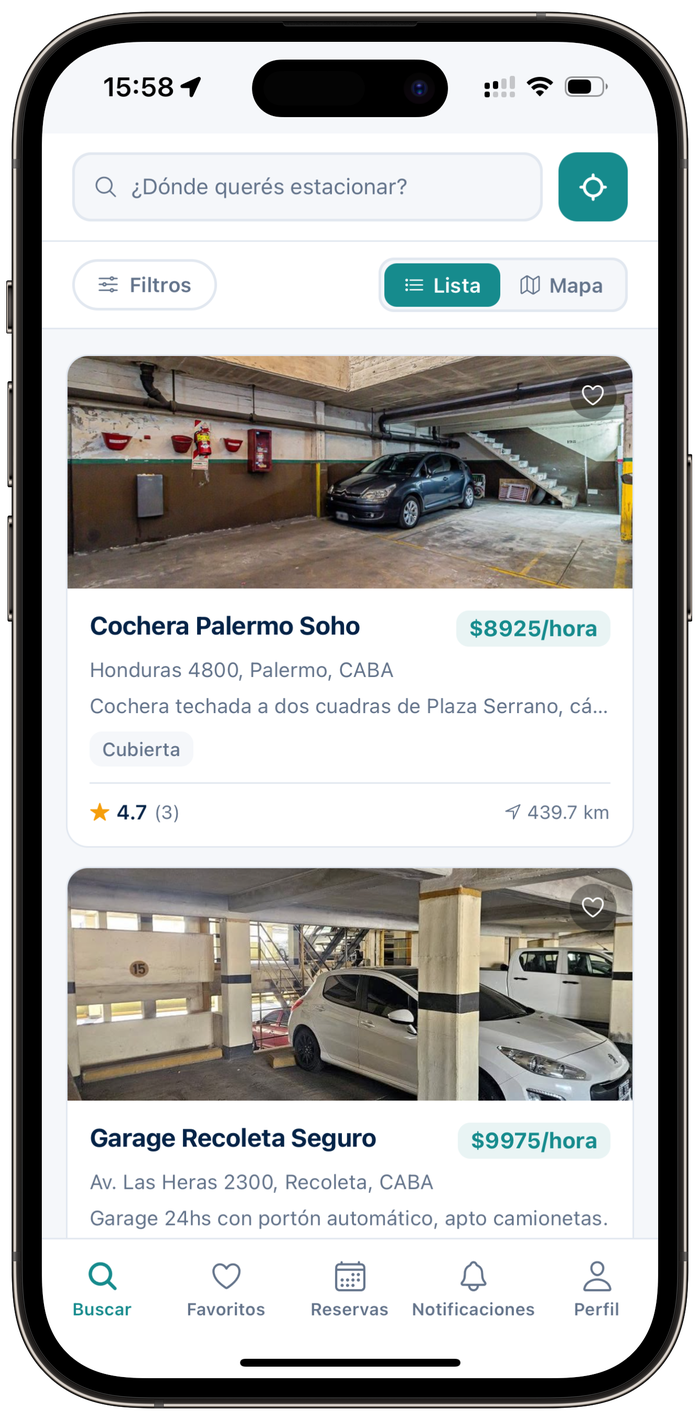
\includegraphics[width=0.158\textwidth]{mockup-8} &
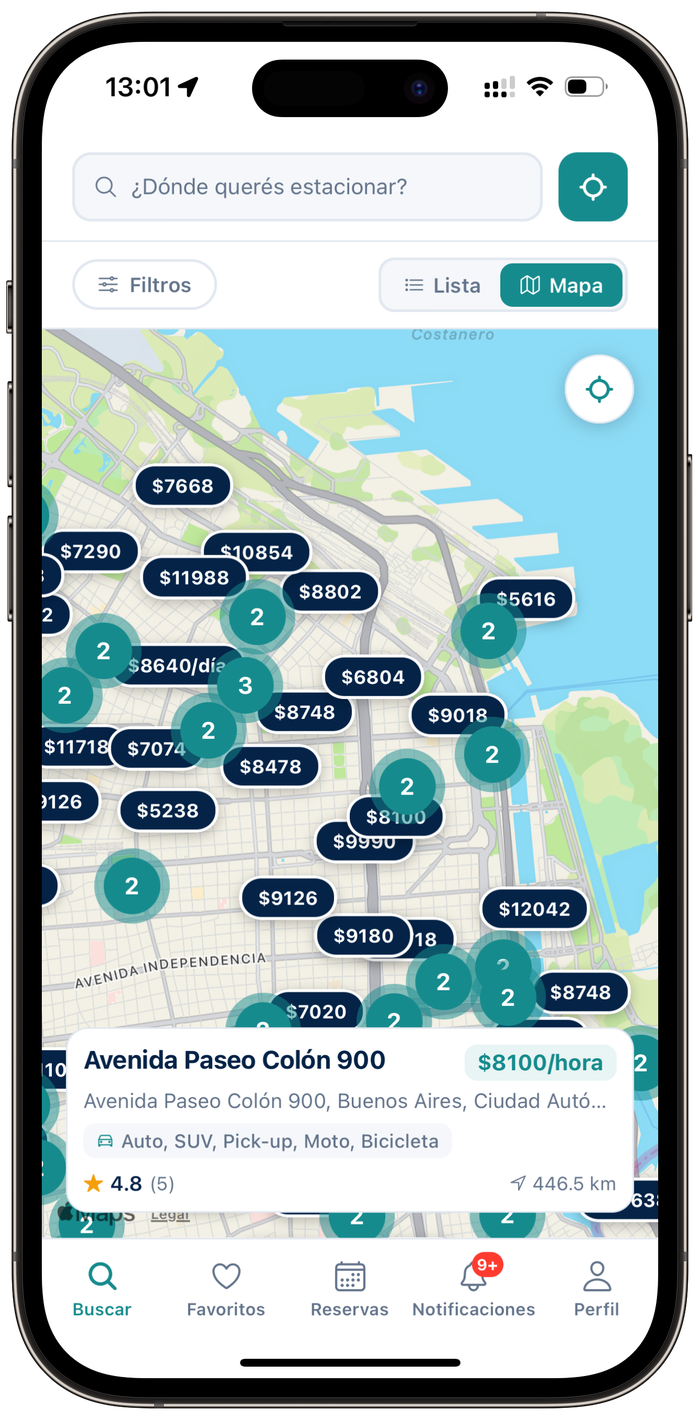
\includegraphics[width=0.158\textwidth]{mockup-22} &
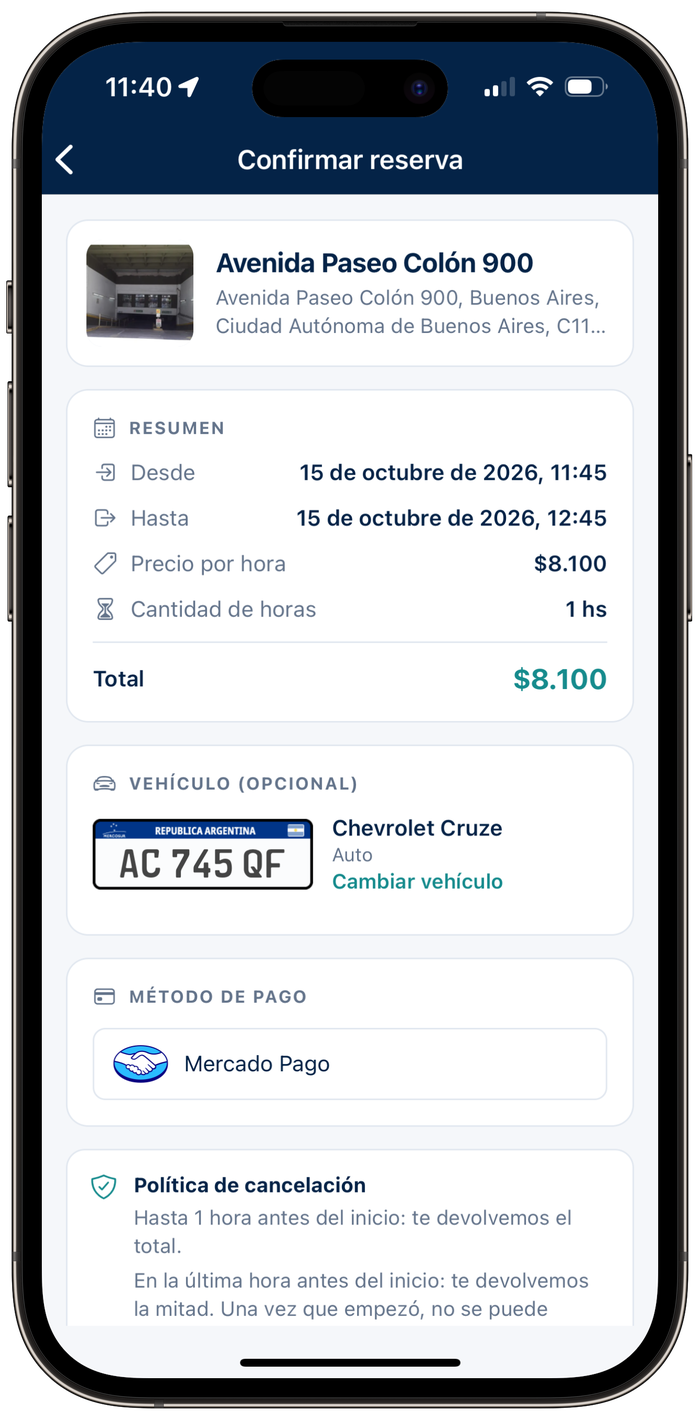
\includegraphics[width=0.158\textwidth]{mockup-25} &
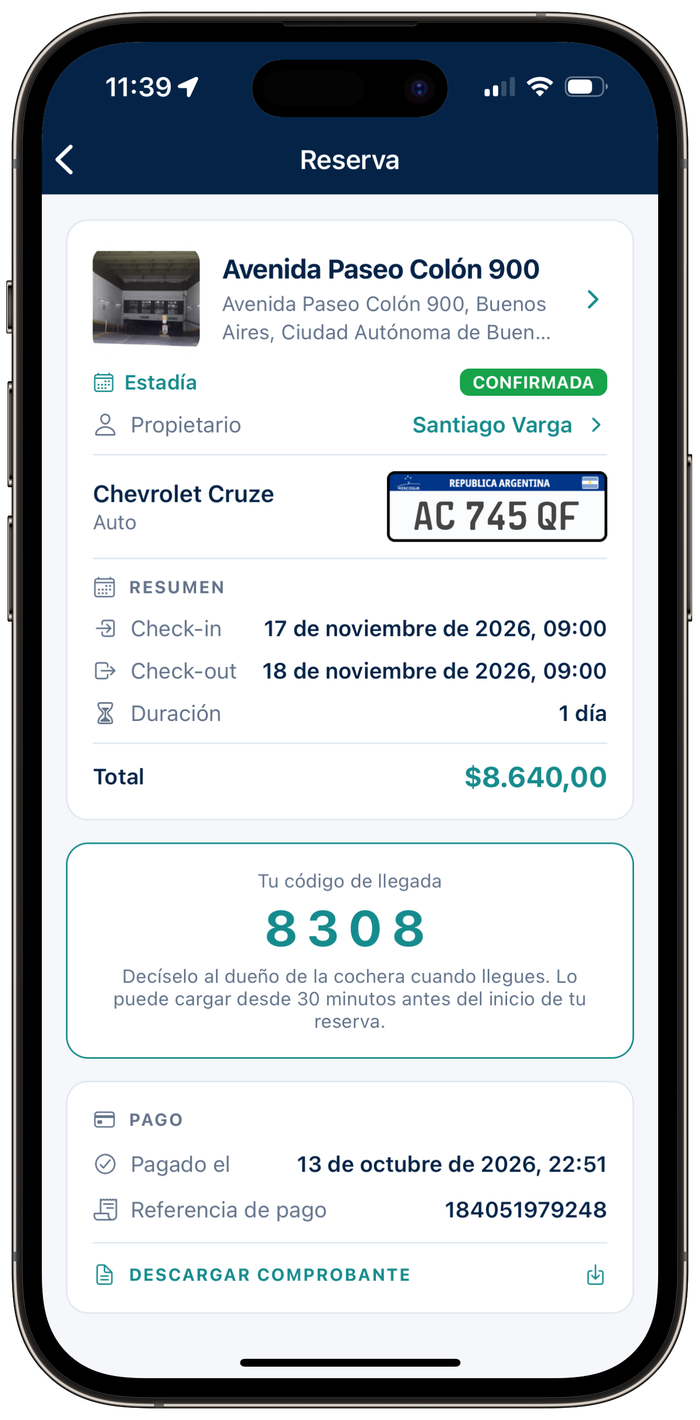
\includegraphics[width=0.158\textwidth]{mockup-23} &
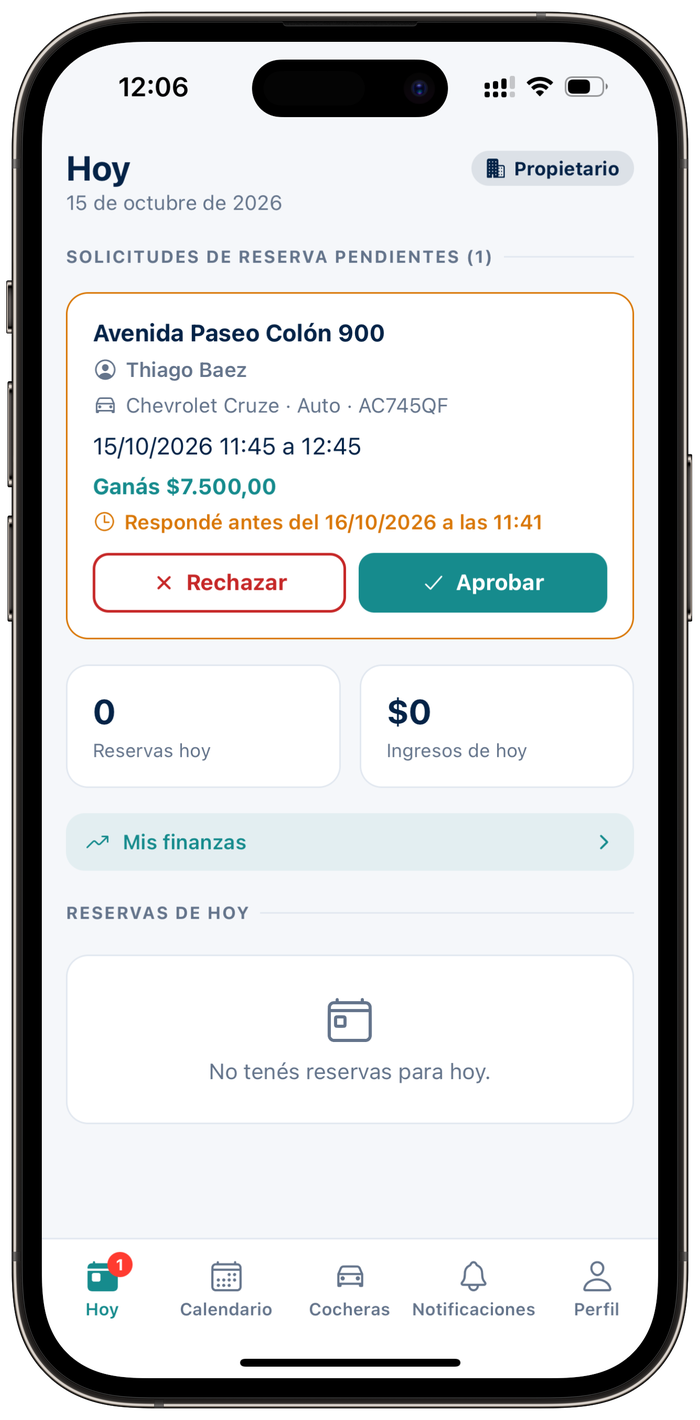
\includegraphics[width=0.158\textwidth]{mockup-38} &
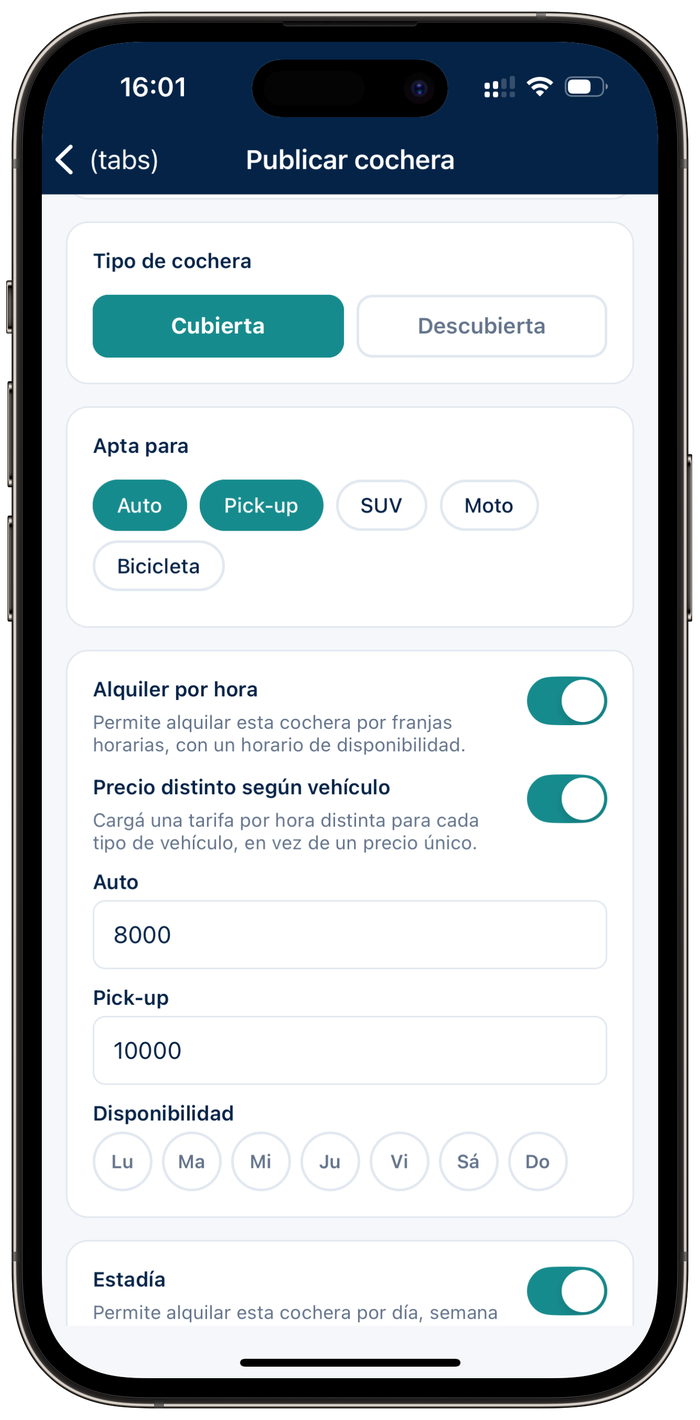
\includegraphics[width=0.158\textwidth]{mockup-10} \\
\footnotesize (a) Lista & \footnotesize (b) Mapa & \footnotesize (c) Confirmación & \footnotesize (d) Código de llegada & \footnotesize (e) Solicitudes & \footnotesize (f) Publicación \\
\end{tabular}
\caption{Aplicación móvil de ParkLink: Búsqueda en lista y en mapa (a, b), confirmación de la reserva (c) y reserva confirmada con su código de llegada (d) en el modo conductor; solicitudes pendientes (e) y publicación de una cochera (f) en el modo propietario.}
\label{fig:app}
\end{figure*}

El panel de administración se convirtió en la sala de operaciones de la plataforma. Su pantalla de inicio resume lo que requiere atención (cocheras por revisar, reservas sin verificar, tickets sin responder, denuncias, reembolsos pendientes y liquidaciones por confirmar) junto con métricas de reservas, facturación, cargo de servicio y reembolsos. Desde allí, el personal modera las publicaciones antes de que aparezcan en las búsquedas, resuelve los pagos retenidos, transfiere las ganancias a los propietarios mediante un flujo de liquidación de tres pasos con comprobante, atiende el soporte, oculta reseñas ofensivas, envía avisos y configura el cargo de servicio sin necesidad de publicar una nueva versión de la aplicación. El acceso se limita a cuentas de personal con dos niveles de permisos.

\subsection{Validación técnica}

Al cierre del desarrollo, el sistema contaba con 128 archivos de pruebas automatizadas, distribuidos como muestra la Tabla~\ref{tab:pruebas}. La distribución refleja dónde se concentra el riesgo: El servicio de reservas, que contiene la mayor parte de las reglas de negocio, reunió el 56\% de los archivos. Los casos críticos verificados de forma automatizada incluyeron el cálculo de disponibilidad en bordes de horarios, cambios de día y conversión horaria; la imposibilidad de sobre-reservar ante solicitudes simultáneas y la expiración de la retención temporal; la generación y validación de los códigos de ingreso y egreso y el cálculo del recargo por permanencia excedida; la verificación de firmas de Mercado Pago, la confirmación idempotente y los reintentos de reembolsos; la deduplicación de eventos y la tolerancia a mensajes malformados; y el rechazo, en la puerta de enlace, de solicitudes sin credenciales o con encabezados internos falsificados. Todas estas pruebas se ejecutaron ante cada cambio en el circuito de integración continua.

\begin{table}[!t]
\centering
\caption{Archivos de pruebas automatizadas por componente}
\label{tab:pruebas}
\renewcommand{\arraystretch}{1.2}
\begin{tabular}{l l r}
\toprule
\textbf{Componente} & \textbf{Marco de pruebas} & \textbf{Archivos} \\
\midrule
Reservas & Go \textit{testing}, \textit{testify}, \textit{gomock} & 72 \\
Notificaciones & \textit{pytest} & 17 \\
Autenticación & \textit{pytest} & 10 \\
Aplicación móvil & \textit{Jest} & 9 \\
Cocheras & \textit{Jest} & 7 \\
Pagos & \textit{Jest}, \textit{supertest} & 7 \\
Puerta de enlace & \textit{pytest} & 6 \\
\midrule
\textbf{Total} & & \textbf{128} \\
\bottomrule
\end{tabular}
\end{table}

Sobre el sistema integrado se ejecutó un \textit{script} de punta a punta que crea un propietario, publica una cochera con horario y precio, crea un conductor, consulta la disponibilidad, genera una reserva y verifica el resultado de cada paso, lo que permitió detectar regresiones después de cada integración. Las pruebas manuales se realizaron sobre teléfonos Android e iOS reales para verificar lo que un emulador no reproduce con fidelidad: La recepción de notificaciones \textit{push}, la ubicación del dispositivo y la redirección al pago de Mercado Pago y el regreso a la aplicación. Los pagos se probaron en el entorno de pruebas de la pasarela, sin movimiento de dinero real, y la búsqueda se evaluó con un generador de datos de demostración con cocheras distribuidas en distintos barrios de CABA. El recorrido completo de búsqueda, reserva, pago y notificación se verificó sin fallas de concurrencia.

\subsection{Riesgos técnicos materializados}

La validación también expuso riesgos que obligaron a revisar decisiones. El más significativo fue de modelo de dominio: El motor de reservas original impedía la superposición de horarios con una restricción de exclusión a nivel de base de datos, que asumía cocheras de un solo lugar y rechazaba reservas válidas en playas comerciales. Se reemplazó por la verificación de capacidad bajo bloqueo pesimista descripta en la Sección~\ref{sec:propuesta}. La dependencia de servicios externos se materializó en las restricciones de la cuenta de prueba de Twilio, en los requisitos para compilar notificaciones \textit{push} en iOS y en los límites de frecuencia de Nominatim, y se mitigó con implementaciones simuladas de cada proveedor en los entornos de desarrollo y con la habilitación temprana de las credenciales productivas. Los \textit{webhooks} de pago, que la pasarela solo envía a direcciones públicas, se probaron mediante túneles seguros. Por último, el entorno distribuido presentó condiciones de carrera en el arranque de los contenedores, resueltas con controles de salud y dependencias condicionales, y fallas de los módulos nativos de notificaciones en el cliente genérico de Expo, resueltas con compilaciones de desarrollo propias mediante EAS~\cite{eas}.

Un riesgo no previsto fue de alcance: El diseño inicial solo contemplaba la aplicación para conductores y propietarios, y al acercarse las pruebas se evidenció que una plataforma de dos lados no puede operar con usuarios reales sin herramientas para moderar publicaciones, resolver disputas y liquidar ganancias. Esto motivó la incorporación del panel de administración al MVP.

\subsection{Validación de mercado}

A principios de septiembre de 2026 se realizó una encuesta difundida por Instagram entre personas de CABA, que obtuvo 180 respuestas. La mayoría correspondió a conductores frecuentes, aunque también participó un grupo numeroso de personas con cocheras libres, lo que permitió relevar ambos lados del mercado. La posibilidad de salir con el lugar ya reservado y pagado fue el aspecto mejor valorado, con calificaciones de 4 o 5 sobre 5 en la gran mayoría de las respuestas, y alrededor del 70\% de los encuestados indicó que usaría la aplicación de forma regular, con frecuencias que van desde algunas veces al mes hasta todos los días. Los motivos más elegidos fueron el precio, conocido de antemano y comparable entre cocheras; la cercanía al destino; y el cuidado del vehículo frente a dejarlo en la calle. El rango de precio que los conductores declararon dispuestos a pagar resultó inferior al promedio de mercado usado en las proyecciones económicas, lo que confirma que el precio es el principal factor de decisión y refuerza la importancia de incorporar cocheras particulares capaces de competir con las playas comerciales.

La encuesta permitió además identificar las fricciones que podían frenar la adopción. Cada una se trató como un riesgo de producto y se resolvió con una decisión implementada antes del lanzamiento, como resume la Tabla~\ref{tab:fricciones}.

\begin{table}[!t]
\centering
\caption{Fricciones detectadas en la validación y decisiones implementadas}
\label{tab:fricciones}
\renewcommand{\arraystretch}{1.2}
\begin{tabular}{>{\raggedright\arraybackslash}p{2.35cm} >{\raggedright\arraybackslash}p{5.3cm}}
\toprule
\textbf{Fricción} & \textbf{Decisión implementada} \\
\midrule
Cochera ocupada por el conductor anterior & Período de gracia de 15 min entre turnos, código de egreso y recargo automático por permanencia excedida \\
\rowcolor{plgray}
Cómo ingresar a una cochera privada & Instrucciones de acceso privadas, visibles solo con la reserva aceptada \\
Cocheras inexistentes o fraudulentas & Moderación previa con documentación de respaldo y verificación de correo y teléfono de todos los usuarios \\
\rowcolor{plgray}
Reglamentos de copropiedad & Declaración del propietario sobre su derecho a ofrecer la cochera en los Términos y Condiciones \\
Propietario que no quiere estar presente & Aprobación con un toque, reembolso automático si no responde, acceso sin su presencia y liquidación periódica \\
\rowcolor{plgray}
Responsabilidad ante daños & Marco de responsabilidades en los Términos y Condiciones, mensajería y tickets de soporte por reserva \\
\bottomrule
\end{tabular}
\end{table}

\subsection{Validación con un referente del sector}

En la última semana de septiembre, ya con el MVP integrado, el equipo se reunió con Miguel Botbol, dueño de Parking Work S.R.L. y de otras empresas del rubro que suman cerca de 70 cocheras en CABA y el conurbano bonaerense. Se le demostraron en vivo la experiencia del conductor, la del propietario y el panel de administración. El encuentro ratificó que la plataforma resulta valiosa no solo para los propietarios particulares, sino también para los operadores comerciales, y que un canal digital que reúna toda la oferta, comercial y particular, con reserva anticipada y pago integrado, responde a una necesidad que el mercado no cubre. Sus aportes sobre la operación cotidiana de las playas orientaron las líneas de trabajo futuro.

\subsection{Validación legal}

Antes de habilitar el uso por personas reales se redactaron y publicaron en el sitio del proyecto los Términos y Condiciones y la Política de Privacidad. Los Términos regulan reservas, pagos, cancelaciones, liquidaciones y responsabilidades, exigen la mayoría de edad y la declaración del propietario sobre su derecho a ofrecer la cochera, y preservan los derechos que la Ley 24.240 de Defensa del Consumidor~\cite{ley24240} reconoce a los usuarios. La Política de Privacidad se elaboró conforme a la Ley 25.326 de Protección de los Datos Personales~\cite{ley25326} y detalla qué datos se recolectan, con qué finalidad, con quién se comparten, cuánto tiempo se conservan y cómo ejercer los derechos de acceso, rectificación y supresión. Su aceptación es un paso obligatorio del registro, y la aplicación permite consultarlos en todo momento y eliminar la propia cuenta.

\subsection{Viabilidad económica}

El modelo económico se construyó sobre un mercado potencial de entre 180.000 y 270.000 búsquedas diarias de estacionamiento en CABA, equivalente al 10--15\% de los vehículos que circulan por la Ciudad. Con un ticket promedio de \$20.000~ARS por reserva, correspondiente a una estadía de dos horas y media, el cargo de servicio del 8\% genera unos USD~1,07 por reserva, a un tipo de cambio de referencia de \$1.500~ARS por dólar. Con una adopción del 0,28\% del mercado en el segundo año (600 reservas diarias), la operación alcanza el punto de equilibrio con un resultado positivo de USD~109.200, que permite recuperar la inversión inicial estimada de USD~69.000. En el largo plazo, con una adopción del 0,91\% (1.966 reservas diarias), la utilidad neta anual proyectada ronda los USD~600.000.

%================================================================
\section{Conclusiones}\label{sec:conclusiones}
%================================================================

\subsection{Conclusiones}

Este trabajo presentó ParkLink, un mercado digital de dos lados que aborda la ineficiencia de la búsqueda de estacionamiento en Buenos Aires. Su aporte central es haber transformado un problema de parada óptima con información incompleta en una elección simultánea entre opciones visibles, comparables y reservables antes de salir, integrando en una única plataforma la búsqueda georreferenciada, la disponibilidad real, el pago y el acceso a la oferta de propietarios particulares, combinación que ningún actor del mercado local ofrecía.

En el plano técnico, la arquitectura de microservicios políglota, con una base de datos por servicio, comunicación por eventos y contratos acordados de antemano, permitió que cuatro personas desarrollaran ocho componentes en paralelo sin bloqueos y que las fallas de un componente secundario no afectaran la operación principal. El motor de reservas resolvió la concurrencia sin sobre-reserva y admitió tanto cocheras particulares como playas comerciales de capacidad múltiple, y la integración de pagos se volvió confiable gracias a la verificación de firmas y al procesamiento idempotente. La metodología híbrida, aplicada de forma distinta en cada fase, ofreció la previsibilidad necesaria a lo largo de trece \textit{sprints} y unas 1.600 horas de trabajo del equipo. La validación confirmó la corrección técnica del sistema, el interés de ambos lados del mercado, el valor de la propuesta para los operadores comerciales y su encuadre en la normativa vigente.

El proyecto integró, además, conocimientos de toda la carrera de Ingeniería en Informática: Los algoritmos de intervalos y las transacciones de bases de datos en el motor de disponibilidad, la programación concurrente en el control de la sobre-reserva, los sistemas distribuidos en la comunicación por eventos y su idempotencia, la ingeniería de software en la metodología y la estrategia de pruebas, y la formación en empresas de base tecnológica en el análisis de mercado y el modelo de ingresos.

\subsection{Lecciones aprendidas}

Tres lecciones resultaron especialmente valiosas. Primero, acordar los contratos entre servicios antes de implementarlos y trabajar contra versiones simuladas fue lo que hizo posible el desarrollo en paralelo. Segundo, una plataforma de dos lados necesita desde el inicio herramientas de operación, como la moderación, la resolución de disputas y las liquidaciones, que no forman parte de la experiencia visible del usuario pero sin las cuales no puede funcionar. Tercero, contrastar el producto temprano con usuarios y con un referente del sector convirtió fricciones que podían frenar la adopción en decisiones concretas de diseño.

\subsection{Trabajo futuro}

Quedaron fuera del alcance del MVP, de forma deliberada, la detección automática de la ocupación y la predicción de la demanda. La primera línea de trabajo consiste en reemplazar la disponibilidad declarada por sensado en tiempo real, mediante visión computacional, reconocimiento automático de patentes para el ingreso sin códigos y sensores IoT comunicados por protocolos livianos como MQTT o LoRaWAN, junto con modelos predictivos de demanda que permitan tarifas dinámicas. La segunda, surgida del encuentro con el referente del sector, es adaptar el motor de reservas y el panel de administración a la operatoria de las grandes playas: Cupos mixtos entre rotativos y abonados mensuales, asignación de pisos y sectores, reglas de precios complejas e integración con las barreras de acceso existentes. La tercera es la expansión a otras ciudades de América Latina y de Estados Unidos, con soporte multimoneda, pasarelas de pago internacionales y adecuación a normas de protección de datos como el RGPD y la CCPA.

%================================================================
\begin{thebibliography}{99}

\bibitem{superauto2024}
SuperAuto, ``¿Cuántos automóviles ingresan diariamente a Capital Federal?'' 2024. [En línea]. Disponible: \url{https://superauto.com.ar/automoviles-que-ingresan-a-capital-federal-por-dia/}

\bibitem{aboy2025movilidad}
R. Aboy, ``La movilidad porteña: Entre aciertos pioneros y el caos diario,'' 2025. [En línea]. Disponible: \url{https://www.iciudad.org.ar/9702-la-movilidad-portena-entre-aciertos-pioneros-y-el-caos-diario/}

\bibitem{ferguson1989}
T.~S. Ferguson, ``Who solved the secretary problem?'' \textit{Statistical Science}, vol.~4, no.~3, pp.~282--289, 1989.

\bibitem{christian2016}
B. Christian y T. Griffiths, \textit{Algorithms to Live By: The Computer Science of Human Decisions}. New York, NY, USA: Henry Holt and Company, 2016.

\bibitem{macqueen1960}
J. MacQueen y R.~G. Miller, Jr., ``Optimal persistence policies,'' \textit{Operations Research}, vol.~8, no.~3, pp.~362--380, 1960.

\bibitem{fergusonstopping}
T.~S. Ferguson, \textit{Optimal Stopping and Applications}, cap.~2, sec.~2.5: ``The parking problem.'' Mathematics Department, University of California, Los Angeles. [En línea]. Disponible: \url{https://www.math.ucla.edu/~tom/Stopping/Contents.html}

\bibitem{tamaki1988}
M. Tamaki, ``Optimal stopping in the parking problem with U-turn,'' \textit{Journal of Applied Probability}, vol.~25, no.~2, pp.~363--374, 1988.

\bibitem{infobae_salarios_2026}
Infobae, ``Provincias líderes, brecha salarial y futuro del empleo: El mapa económico de la Argentina,'' 2026. [En línea]. Disponible: \url{https://www.infobae.com/economia/2026/05/03/provincias-lideres-brecha-salarial-y-futuro-del-empleo-el-mapa-economico-de-la-argentina-segun-6-indicadores-clave/}

\bibitem{economista_nafta_2026}
El Economista, ``Precio de la nafta hoy: Cuánto cuesta el litro en marzo de 2026,'' 2026. [En línea]. Disponible: \url{https://eleconomista.com.ar/energia/precio-nafta-hoy-cuanto-cuesta-litro-marzo-2026-n93548}

\bibitem{infobae_multas_2026}
Infobae, ``Aumentaron las multas de tránsito en la Ciudad de Buenos Aires: El ranking de las infracciones más caras,'' 2026. [En línea]. Disponible: \url{https://www.infobae.com/sociedad/2026/03/07/aumentaron-las-multas-de-transito-en-la-ciudad-de-buenos-aires-el-ranking-de-las-infracciones-mas-caras/}

\bibitem{iprofesional2026cocheras}
R. Ramallo, ``Cuánto cuesta estacionar en CABA: Hay zonas donde cobran hasta \$20.000 por hora y una cochera supera los \$300.000 por mes,'' \textit{iProfesional}, 6 jul. 2026. [En línea]. Disponible: \url{https://www.iprofesional.com/autos/459287-cuanto-cuesta-estacionar-en-caba-hay-zonas-donde-cobran-hasta-20000-por-hora}

\bibitem{shoup2005}
D.~C. Shoup, \textit{The High Cost of Free Parking}. Chicago, IL, USA: Planners Press, American Planning Association, 2005.

\bibitem{shoup2006}
D.~C. Shoup, ``Cruising for parking,'' \textit{Transport Policy}, vol.~13, no.~6, pp.~479--486, 2006.

\bibitem{blinkay}
Blinkay, ``Blinkay: Estacionamiento medido en Argentina,'' 2026. [En línea]. Disponible: \url{https://www.blinkay.com}

\bibitem{waze}
Waze, ``Waze: Free community-based GPS navigation app,'' 2026. [En línea]. Disponible: \url{https://www.waze.com}

\bibitem{googlemaps}
Google LLC, ``Google Maps,'' 2026. [En línea]. Disponible: \url{https://maps.google.com}

\bibitem{mercadolibre}
Mercado Libre, ``Mercado Libre: Plataforma de compraventa online,'' 2026. [En línea]. Disponible: \url{https://www.mercadolibre.com.ar}

\bibitem{spothero}
SpotHero, ``SpotHero: Find and reserve parking online,'' 2026. [En línea]. Disponible: \url{https://spothero.com}

\bibitem{easypark}
EasyPark Group, ``EasyPark: Smart parking solutions,'' 2026. [En línea]. Disponible: \url{https://easyparkgroup.com}

\bibitem{mercadopago}
Mercado Pago, ``Mercado Pago Developers: Documentación oficial,'' 2026. [En línea]. Disponible: \url{https://www.mercadopago.com.ar/developers}

\bibitem{firebase}
Google LLC, ``Firebase Cloud Messaging: Documentación oficial,'' 2026. [En línea]. Disponible: \url{https://firebase.google.com/docs/cloud-messaging}

\bibitem{reactnative}
Meta Open Source, ``React Native,'' 2026. [En línea]. Disponible: \url{https://reactnative.dev}

\bibitem{expo}
Expo, ``Expo: Documentación oficial,'' 2026. [En línea]. Disponible: \url{https://docs.expo.dev}

\bibitem{brevo}
Brevo, ``Brevo: Documentación para desarrolladores,'' 2026. [En línea]. Disponible: \url{https://developers.brevo.com}

\bibitem{twilio}
Twilio Inc., ``Twilio Programmable Messaging: Documentación oficial,'' 2026. [En línea]. Disponible: \url{https://www.twilio.com/docs/messaging}

\bibitem{nominatim}
OpenStreetMap Foundation, ``Nominatim: Geocodificación sobre datos de OpenStreetMap,'' 2026. [En línea]. Disponible: \url{https://nominatim.org}

\bibitem{cloudflarer2}
Cloudflare, Inc., ``Cloudflare R2: Documentación oficial,'' 2026. [En línea]. Disponible: \url{https://developers.cloudflare.com/r2/}

\bibitem{sentry}
Functional Software, Inc., ``Sentry: Documentación oficial,'' 2026. [En línea]. Disponible: \url{https://docs.sentry.io}

\bibitem{docker}
Docker, Inc., ``Docker: Documentación oficial,'' 2026. [En línea]. Disponible: \url{https://docs.docker.com}

\bibitem{rabbitmq}
Broadcom Inc., ``RabbitMQ: Reliable messaging and streaming broker,'' 2026. [En línea]. Disponible: \url{https://www.rabbitmq.com}

\bibitem{githubactions}
GitHub, Inc., ``GitHub Actions: Documentación oficial,'' 2026. [En línea]. Disponible: \url{https://docs.github.com/actions}

\bibitem{cloudflaretunnel}
Cloudflare, Inc., ``Cloudflare Tunnel: Documentación oficial,'' 2026. [En línea]. Disponible: \url{https://developers.cloudflare.com/cloudflare-one/connections/connect-networks/}

\bibitem{eas}
Expo, ``EAS Build: Expo Application Services,'' 2026. [En línea]. Disponible: \url{https://docs.expo.dev/build/introduction/}

\bibitem{ley24240}
Honorable Congreso de la Nación Argentina, ``Ley N.º 24.240 de Defensa del Consumidor,'' B.O. 15/10/1993. [En línea]. Disponible: \url{https://servicios.infoleg.gob.ar/infolegInternet/anexos/0-4999/638/texact.htm}

\bibitem{ley25326}
Honorable Congreso de la Nación Argentina, ``Ley N.º 25.326 de Protección de los Datos Personales,'' B.O. 02/11/2000. [En línea]. Disponible: \url{https://servicios.infoleg.gob.ar/infolegInternet/anexos/60000-64999/64790/norma.htm}

\end{thebibliography}

\end{document}
